\chapter*{Introduction}
\addtocontents{toc}{\protect\vspace{\beforebibskip}} % to have the bib a bit from the rest in the toc
\addcontentsline{toc}{section}{\tocEntry{Introduction}}

\epigraph{
pity this busy monster, manunkind,
    }{
    --- \textsc{E. E. Cummings}}

This will be the subject of Chapter \ref{ch:QM}

\todo[inline]{CURRENTLY VERBATIM FROM MASTER THESIS}
A similar situation in encountered when quantum chemistry deals with the
description of complex systems, such as solutions or proteins. Unlike
relativity, the inclusion of the environment in the description of a
chemical system has been considered from the early stages in the
evolution of quantum chemistry.
Already in 1936 \citeauthor{Onsager1936-wf} had proposed a model to
account for the presence of a liquid on point-like electric
moments.~\autocite{Onsager1936-wf}

As the development of our knowledge of solutions reflects to some extent
the development of chemistry itself, this interest is very well
justified.
Despite the large number of reactions known to happen in the solid state
and in gas phase, we can state that almost always chemistry happens in
solution.~\autocite{Reichardt2010-le}

The theoretical treatment of environment effects suffers from a
\emph{dimensionality} problem, since even the most simplified picture of
the system under consideration would require taking into account
500--1000 atoms, at least. Application of the most accurate methods in
quantum chemistry is therefore impossible and not even desirable: as
always in problems with a high dimensionality, the microscopic detail in
the physical description cannot account for the macroscopic behaviour of
the system. This is an important point that will be discussed in greater
detail later.
Models must be devised to overcome the dimensionality ``disease'': the
ability to account, at least qualitatively, for environment effects is
rather fundamental in all experimental branches of
chemistry.~\autocite{Anderson1972-ai, Winsberg2010-sy, Kovac2011-ew}

\section*{The Problem of Solvation or Taming Complexity with Models}

\todo[inline]{CURRENTLY VERBATIM FROM MASTER THESIS}

We should state more precisely what we mean by solution, here and in the
following we will always refer to a system were the number of solvent
molecules exceeds by far the number of solute molecules. From an
experimental point of view, it is an \emph{extremely} dilute solution.
We will follow the expositions given by Tomasi in refs.~
\noparcite{Tomasi2004-dc} and \noparcite{Tomasi2007-es}.

Our observables of interest are the same as \emph{in vacuo}, \ie
relative energies, spectroscopic parameters and so forth. These
observables are influenced by the presence of the solvent and this is
what is commonly called \emph{solvent effect}.
Solvent effects are, customarily but conveniently, classified as:
\begin{itemize}
\item[.] \emph{direct}. The presence of the solvent modifies the solute
  electronic density, all observables depending on the density are
  accordingly perturbed;
\item[.] \emph{indirect}. In the Born--Oppenheimer picture the
  electronic energy acts as \ac{PES} for the
  nuclear motion. The most striking solvent effect is thus the
  modification of the equilibrium geometry of a molecular solute.
  Aminoacids are notable examples of this behaviour, exhibiting
  different predominant conformers in different solvents;
\item[.] \emph{local field}. The presence of the solvent can alter the
  response of the system to applied fields, locally modifying the
  applied field itself.~\autocite{Cammi1998-jp, Pipolo2014-sd}
\item[.] \emph{dynamic}. When considering electronic excitations we
  always work in a Franck--Condon framework. This is also true for
  excitation processes in solution. In addition, we will have to
  consider not only the geometric relaxation of the solute, but also the
  relaxation of the surrounding medium;
\item[.] \emph{specific}. A brief description of specific solvent
  effects is not possible, due to their extremely varied nature. The
  name specific comes from the fact that their existence depends on the
  particular solute-solvent pair, rather than only on one of the
  partners. It appears thus safe to say that all the effects that must
  be described considering the atomistic nature of the solute-solvent
  interaction are specific.
\end{itemize}

It is, again, customary and convenient to divide the models proposed in
two classes, according to the microscopic description of the solvent
these models give. Hence we distinguish between:
\begin{itemize}
 \item[.] \emph{discrete} (or \emph{explicit}). The degrees of freedom
   associated with the solvent molecules are dealt with explicitly as
   are those associated with the solute. The two sets of coordinates can
   be treated at different levels of theory;
 \item[.] \emph{continuum} (or \emph{implicit}). Only the degrees of
   freedom associated with the solute are dealt with explicitly, the
   solvent being replaced with a structureless continuum characterized
   by its bulk properties.
\end{itemize}

Continuum models arise as limits, in a proper sense, to the discrete
models. To stress this point we introduce the \emph{solution}
Hamiltonian in the Born--Oppenheimer approximation as:
\begin{equation}\label{eq:solution-ham}
 H(\vect{r}_\mathrm{M}, \vect{r}_\mathrm{S}) =
  H_\mathrm{M}(\vect{r}_\mathrm{M}) +  H_\mathrm{S}(\vect{r}_\mathrm{S})
+ H_\mathrm{MS}(\vect{r}_\mathrm{M}, \vect{r}_\mathrm{S})
\end{equation}
where the subscript M refers to the solute while S to the solvent. The
coordinates $(\vect{r}_\mathrm{M}, \vect{r}_\mathrm{S})$ refer to
\emph{both} nuclei and electrons, the interaction term is given by the
usual Coulombic electrostatic Hamiltonian.

It is important to remark that nuclear coordinates must be considered
explicitly. Liquid phases are, by definition, characterized by the high
mobility of their molecular constituents. Changes in the internal
geometry of solvent molecules, triggered by intermolecular interactions
between themselves and with the solute, always play a role in the
solvation process. Whether this role is prominent or not cannot be
decided \emph{a priori}.

From a computational point of view, using the Hamiltonian in Eq.~\eqref{eq:solution-ham} is simply not feasible. We would have to
determine a \acs{PES} of enormous dimensionality and then explore the full
dynamics of the system. Even assuming that the minimum energy
conformation on the \acs{PES} can be fully characterized, its knowledge will
not lead us to a correct description of the physics of solvation. In
fact, macroscopic observables of systems with a large number of degrees
of freedom arise as \emph{average} values of the microscopic behaviour
of every single component, the average being either on the phase space
trajectory or on the appropriate ensemble.~\autocite{Hill1960-ql}. It is always
necessary to perform some kind of average upon the energies
corresponding to all the accessible conformations of the whole
solute+solvent system.

Of course, this formidable task may be accomplished using statistical
thermodynamics and the idea of \emph{statistical ensembles} developed by
Gibbs. To apply the idea of an ensemble average we must resort to a
molecular dynamics or Monte Carlo simulation of the solution, in order
to obtain the appropriate partition function, $Z$. This introduces a
number of points that will be central in the development of continuum
models:
\begin{enumerate}
 \item statistical simulations rely on \emph{macroscopic} parameters
   such as the temperature or the density. These parameters are not
   present in the Hamiltonian \eqref{eq:solution-ham}, but are necessary
   for the description of molecular systems in the condensed phase. This
   is true whether one considers discrete or continuum approaches;
 \item the basic energetic quantity is the thermodynamic potential
   characterizing the chosen ensemble. If a direct comparison with the
   experiment is sought, one should run a simulation in the $(NpT)$
   ensemble whose potential is the Gibbs free energy $G$. This point is
   of paramount importance in continuum models and we will have the
   opportunity to stress it in this Chapter as well as in Chapter
   \ref{chap:relpcmscf};
 \item even starting from a completely atomistic point of view, our
   final results will always be in the form of an average over solvent
   conformations. We have explicitly replaced a discrete description
   with a continuous distribution function. Atomistic details can of
   course be recovered by further analysis, but the point remains:
   properties of solutions (the solvation energy among them) have an
   intrinsic average nature.
\end{enumerate}

The fact that an averaging procedure is essential in studying solvation
processes should convince the reader that, at least from a purely
mathematical point of view, we can replace the full Hamiltonian
\eqref{eq:solution-ham} with an \emph{effective} Hamiltonian, averaging
the solvent degrees of freedom in a preliminary
step.~\autocite{Angyan1992-vo, Tapia1992-pu}
\todo[inline]{Some pieces missing here, FILL IN}
Alternatively, an approximate decoupling can be obtained replacing the
mean-field operator in Eq.~\eqref{eq:ave1} by its classical average over
a suitable ensemble:
\begin{equation}\label{eq:ave_classic}
 \Braket{H_\mathrm{MS}}_\mathrm{S} = \frac{\int\diff\Gamma H_\mathrm{MS}\exp
\left(-\beta H_\mathrm{S}\right)}{\int\diff\Gamma\exp\left(-\beta H_\mathrm{S}\right)}.
\end{equation}
This classical average can be written in terms of the $g(\vect{r})$ distribution functions. These functions are defined
for the electrons and the nuclei of the solvent with respect to the fixed frame of reference of the solute molecule, see \noparcite[ref.][]{hansen}.
This amounts to considering the solvent as a structureless continuum, hence defining continuum models.

Continuum models are then characterized, by a solute-only
\emph{effective} Hamiltonian:\footnote{We will use the symbol
$H_\mathrm{MS}$ for the interaction Hamiltonian even if it is not the
full interaction term of Eq.~\eqref{eq:solution-ham}.}
\begin{equation}\label{eq:effective-ham}
 H(\vect{r}_\mathrm{M}) = H_\mathrm{M}(\vect{r}_\mathrm{M})
+ H_\mathrm{MS}(\vect{r}_\mathrm{M}),
\end{equation}
the explicit form of the averaged interaction in
Eq.~\eqref{eq:effective-ham} is in terms of solvent \emph{response
functions}, $Q_x(\vect{r},\vect{r}^\prime)$.
As will be apparent in the following, this term may depend on the solute
density, making the effective Hamiltonian \emph{nonlinear}.

An hierarchy of approximations for the resolution of the effective
Schr\"odinger equation can be devised, as was done for the discrete
models. The distinguishing feature is now the \emph{order} of the
solvent response functions used in the definition of the interaction
term.

If we limit ourselves to a linear response of the solvent we obtain the
class of models commonly called continuum solvation models, the
Polarizable Continuum Model among them. Computer simulations can be used
to determine these functions, but almost always one uses bulk properties
of the pure solvent obtained from experiment.

This, at first sight, crude approximation is rather well justified by
the following argument: from a physical point of view, our solution is
extremely dilute. The presence of the solute is an extremely small
perturbation for the bulk of the solvent and it is safe to assume that
the macroscopic properties of the solution are not far from those of the
pure solvent. Furthermore, the use of macroscopic experimental values
implicitly takes into account the averaging procedure one would carry
out in atomistic simulations of the solution.

As pictorially represented in Figure \ref{fig:discretetocontinuum} the
solvent is now a \emph{structureless polarizable} continuum and the
solute is accommodated inside a cavity formed in this continuum.
\begin{figure}[!h]
 \centering
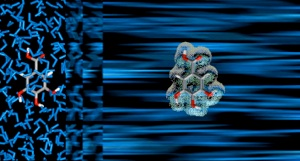
\includegraphics[width=.5\textwidth]{discretetocontinuum}
\caption{Pictorial representation of the transition from a discrete to a
continuum model of a solution.}
\label{fig:discretetocontinuum}
\end{figure}

\autocite{Anderson1972-ai}

This will be the subject of Chapter \ref{ch:CSM}

\section*{The Road to Reality or Molecular Response Properties}

This will be the subject of Chapter \ref{ch:molprop}

\section*{Accurate Methods for Accurate Properties}

This will be the subject of Chapter \ref{ch:solvation-correlation}
